\documentclass[a4paper,10pt]{article}

\usepackage{listings}

%Math
\usepackage{amsmath}
\usepackage{amsfonts}
\usepackage{amssymb}
\usepackage{amsthm}
\usepackage{ulem}
\usepackage{stmaryrd} %f\UTF{00FC}r Blitz!

%PageStyle
\usepackage[german]{babel}
\usepackage{fontenc}
\usepackage{fancyhdr, graphicx}
\usepackage{wasysym}
\usepackage{fullpage}
\usepackage{textcomp}
\usepackage{fancyhdr} %for header/footer

%My Commands
\newcommand{\BN}{\mathbb{B}} %BOOL
\newcommand{\RN}{\mathbb{R}} %Real Number
\newcommand{\NN}{\mathbb{N}} %Natural Number
\newcommand{\QN}{\mathbb{Q}} %Rational Number
\newcommand{\ZN}{\mathbb{Z}} %ganze Zahlen
\newcommand{\CN}{\mathbb{C}}
\newcommand{\Teilt}{\mid} %|
\newcommand{\Teiltn}{\nmid} %kein teiler
\newcommand{\Potp}{\mathcal{P}} %Potenzmenge
\newcommand{\Pota}{\mathcal{A}}
\newcommand{\Potr}{\mathcal{R}}
\newcommand{\Potn}{\mathcal{N}}
\newcommand{\Bold}[1]{\textbf{#1}} %Boldface
\newcommand{\Kursiv}[1]{\textit{#1}} %Italic
\newcommand{\T}[1]{\text{#1}} %Textmode
\newcommand{\Nicht}[1]{\T{\sout{$ #1 $}}} %Streicht Shit durch
\newcommand{\lra}{\leftrightarrow} %Arrows
\newcommand{\ra}{\rightarrow}
\newcommand{\la}{\leftarrow}
\newcommand{\lral}{\longleftrightarrow}
\newcommand{\ral}{\longrightarrow}
\newcommand{\lal}{\longleftarrow}
\newcommand{\Lra}{\Leftrightarrow}
\newcommand{\Ra}{\Rightarrow}
\newcommand{\La}{\Leftarrow}
\newcommand{\Lral}{\Longleftrightarrow}
\newcommand{\Ral}{\Longrightarrow}
\newcommand{\Lal}{\Longleftarrow}
\newcommand{\Vektor}[1]{\vec{#1}}
\newcommand{\Brace}[1]{\left( #1 \right)} %()
\newcommand{\Bracel}[1]{\left\lbrace #1 \right.} %(
\newcommand{\Bracer}[1]{\right. #1 \right\rbrace} %)
\newcommand{\Brack}[1]{\left\lbrace #1 \right\rbrace} %{}
\newcommand{\Brackl}[1]{\left\lbrace #1 \right.} %{
\newcommand{\Brackr}[1]{\right. #1 \right\rbrace} %}
\newcommand{\Result}[1]{\underline{\underline{#1}}} %Doppelt unterstrichen
\newcommand{\Abs}[1]{\left| #1 \right|} %Absolutbetrag
\newcommand{\Norm}[1]{\Abs{\Abs{ #1 }}} %Norm
\newcommand{\Arrays}[1]{\left(\begin{array}{c}#1\end{array}\right)} %Array mit einer Kolonne ()
\newcommand{\Array}[2]{\left(\begin{array}{#1}#2\end{array}\right)} %Array mit n Kolonnen ()
\newcommand{\Bracka}[2]{\left\lbrace\begin{array}{#1}#2\end{array}\right\rbrace} %Array mit {}
\newcommand{\Brackal}[2]{\left\lbrace\begin{array}{#1} #2 \end{array}\right.} %Array mit {
\newcommand{\Brackar}[2]{\left.\begin{array}{#1} #2 \end{array}\right\rbrace} %Array mit }
\newcommand{\Sumone}[2]{\sum_{#2=1}^{#1}} %Summe von 1
\newcommand{\Sumz}[2]{\sum_{#2=0}^{#1}} %Summe von 0
\newcommand{\Sum}[2]{\sum_{#2}^{#1}} %Allgemeine Summe
\newcommand{\Oneover}[1]{\frac{1}{#1}} %1 \UTF{00FC}ber igendwas
\newcommand{\Tablewt}[3]{\begin{table*}[h]\caption{#1} \begin{tabular}{#2}{#3}\end{tabular}\end{table*}} %Table mit Titel
\newcommand{\Oben}[2]{\overset{#1}{#2}} %etwas \UTF{00FC}ber etwas anderem
\newcommand{\Unten}[2]{\underset{#1}{#2}} %etwas unter etwas anderem
\newcommand{\Bildcap}[2]{\begin{figure}[htb]\centering\includegraphics[width=0.2\textwidth]{#1} \caption{#2}\end{figure}} %Bild mit beschriftung
\newcommand{\Bildjpeg}[1]{\includegraphics[width=0.2\textwidth]{#1.jpeg}} %Bilder jpeg!!
\newcommand{\Bildjpg}[1]{\includegraphics[width=0.2\textwidth]{#1.jpg}} %Bilder jpg!!

%Zeichnung
\usepackage{tikz}
\usepackage[all]{xy}
\usepackage{ucs}

\definecolor{dkgreen}{rgb}{0,0.6,0}
\definecolor{gray}{rgb}{0.5,0.5,0.5}
\definecolor{mauve}{rgb}{0.58,0,0.82}
 
\lstset{ %
  language=Octave,                % the language of the code
  basicstyle=\footnotesize,           % the size of the fonts that are used for the code
  numbers=left,                   % where to put the line-numbers
  numberstyle=\tiny\color{black},  % the style that is used for the line-numbers
  stepnumber=1,                   % the step between two line-numbers. If it's 1, each line 
                                  % will be numbered
  numbersep=5pt,                  % how far the line-numbers are from the code
  backgroundcolor=\color{white},      % choose the background color. You must add \usepackage{color}
  showspaces=false,               % show spaces adding particular underscores
  showstringspaces=false,         % underline spaces within strings
  showtabs=false,                 % show tabs within strings adding particular underscores
  tabsize=2,                      % sets default tabsize to 2 spaces
  captionpos=b,                   % sets the caption-position to bottom
  breaklines=true,                % sets automatic line breaking
  breakatwhitespace=false,        % sets if automatic breaks should only happen at whitespace
  keywordstyle=\color{blue},          % keyword style
  commentstyle=\color{black},       % comment style
  stringstyle=\color{mauve},         % string literal style
  morekeywords={int,long,float,public,static,class}               % if you want to add more keywords to the set
}

%Config
\renewcommand{\headrulewidth}{0pt}
\setlength{\headheight}{15.2pt}
\pagestyle{plain}

%Metadata
\title{Software-Konstruktion}
\author{Jan F\"assler}
\date{2. Semester (FS 2012)}
\fancyfoot[C]{Jan F\"assler}

\begin{document}
\maketitle
\newpage
\thispagestyle{fancy} %f\UTF{00FC}r Header

\section{Build Automation}
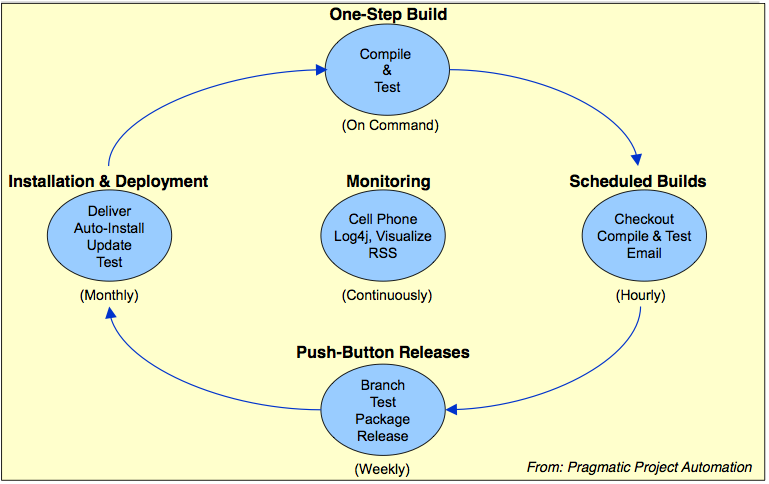
\includegraphics[scale=0.6]{build_automation.png}

\subsection{CRISP Builds}
\begin{description}
	\item[Complete] recipe lists all ingredients
	\item[Repeatable] version control time machine
	\item[Informative] radiate valuable information
	\item[Schedulable] complete and repeatable
	\item[Portable] machine-independent
\end{description}

\subsection{Ant-Script}
\begin{lstlisting}
<project name="Software Construction Lab" default="compile" basedir="..">
    <property file="build/build.properties" />
	
    <!-- The application's classpath -->
    <path id="application.classpath">
        <fileset dir="${lib.dir}">
            <include name="**/*.jar"/>
        </fileset>
    </path>
    
    <!-- The build tools classpath -->
    <path id="build.classpath">
        <fileset dir="${build.lib.dir}">
            <include name="*.jar" />
        </fileset>
        <path refid="application.classpath"/>
    </path>
	
    <target name="clean">
    	<delete dir="${bin}"/>
    	<delete dir="${log}"/>
    </target>
	
    <target name="prepare" depends="clean">
        <mkdir dir="${bin.classes.dir}" />
        <mkdir dir="${bin.jar.dir}" />
        <mkdir dir="${log.report.dir}"/>
    	<mkdir dir="${log.report.test.dir}" />
    	<mkdir dir="${log.report.checkstyle.dir}"/>
    </target>

    <target name="compile" depends="prepare" description="Compile the sources">
        <javac includeantruntime="false" srcdir="${src.dir}" destdir="${bin.classes.dir}" classpathref="application.classpath" deprecation="on" optimize="off"/>
        <copy todir="${bin.classes.dir}">
            <fileset dir="${res.dir}">
                <include name="**/*.xml" />
                <include name="**/*.properties" />
                <include name="**/*.png" />
            </fileset>
        </copy>
    </target>

    <target name="run" depends="jar" description="Run distributed application from jar file">
        <java jar="${bin.jar.dir}/${name}-${version}.jar" fork="true" />
    </target>

    <target name="jar" depends="junit" description="Create jar distribution">
        <jar jarfile="${bin.jar.dir}/${name}-${version}.jar" basedir="${bin.classes.dir}" excludes="**/*Test.class">
            <manifest>
                <attribute name="Main-Class" value="${main.class}" />
                <attribute name="Class-Path" value=".
                    ../../lib/dbunit-2.2.jar
                    ../../lib/hsqldb.jar" />  
            </manifest>
        </jar>
    </target>
	
	<target name="testcompile" depends="compile" description="Compiles JUnit Tests">
		<echo message="Compile Tests" />
		<javac includeantruntime="false" srcdir="${test.dir}" destdir="${bin.classes.dir}" classpathref="build.classpath" deprecation="on" optimize="off"/>
		<echo message="Copy compiled classes to bin directory" />
		<copy todir="${bin.classes.dir}">
            <fileset dir="${res.dir}">
                <include name="**/*.xml" />
                <include name="**/*.properties" />
                <include name="**/*.png" />
            </fileset>
            <fileset dir="${test.dir}">
                <include name="**/*.xml" />
            </fileset>
        </copy>
	</target>
	
	<target name="junit" depends="testcompile" description="Runs JUnit Tests">
       <junit haltonfailure="yes" printsummary="yes">
        	<classpath>
        		<path refid="build.classpath"/>
        		<pathelement location="${bin.classes.dir}" />
        	</classpath>
        	<formatter type="xml"/>
            <batchtest fork="true" todir="${log.report.test.dir}">
                <fileset dir="${test.dir}" includes="**/*Test.java"/>
            </batchtest>
        </junit>
	</target>
	
	<target name="javadoc" depends="prepare" description="Creates the javadoc">
		<delete dir="${doc.api.dir}"/>
	  	<javadoc sourcepath="${src.dir}" destdir="${doc.api.dir}" windowtitle="${name} API">
	    	<doctitle><![CDATA[<h1>${name} API</h1>]]></doctitle>
	    	<bottom><![CDATA[<i>Copyright &#169; 2012 Dummy Corp. All Rights Reserved.</i>]]></bottom>
		    <tag name="todo" scope="all" description="To do:"/>
		    <link offline="true" href="http://download.oracle.com/javase/6/docs/api/" packagelistLoc="C:\tmp"/>
	    	<link href="http://developer.java.sun.com/developer/products/xml/docs/api/"/>
	  	</javadoc>
	</target>
	
	<taskdef resource="checkstyletask.properties" classpath="${build.lib.dir}/checkstyle-5.5-all.jar" />
	<target name="checkstyle" depends="compile" description="Generates a report of code convention violations.">
		<checkstyle config="${build.dir}/swc_checks.xml">
			<fileset dir="${src.dir}" includes="**/*.java"/>
			<classpath>
				<pathelement location="${bin.classes.dir}"/>
			</classpath>
	  		<formatter type="xml" tofile="${log.report.checkstyle.dir}/checkstyle_report.xml"/>
	  		<formatter type="plain" tofile="${log.report.checkstyle.dir}/checkstyle_report.txt"/>
	  		<formatter type="plain" />
		</checkstyle>
	</target>
	
	<target name="all" depends="checkstyle,javadoc,jar"/>

</project>
\end{lstlisting}

\newpage
\section{Continuous Integration}
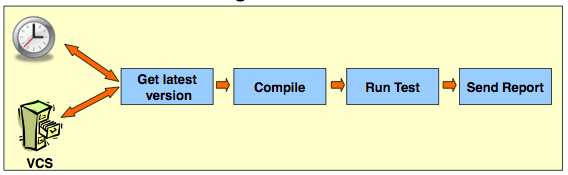
\includegraphics[scale=0.8]{continuous_integration.png}
\begin{itemize}
	\item Maintain a single source repository.
	\item Automate the build
	\item Make your build self-testing
	\item Everyone commits every day (at least!)
	\item Every commit should build the mainline on an integration machine
	\item Keep the build fast
	\item Test in a clone of the production environment	
	\item Make it easy for anyone to get the latest executable
	\item Everyone can see what's happening
	\item Automate deployment
\end{itemize}

\subsection{Benefits}
\begin{itemize}
	\item Reduced Risks
	\item Always be aware of current status of the project
	\item Less time spent investigating integration bugs
		\begin{itemize}
			\item Integration testing performed early
			\item Integration bugs caught early
		\end{itemize}
	\item Less time wasted because of broken code in version control system
	\item Prove your system can build!
	\item Increase code quality with additional tasks
	\item Discover potential deployment issues
\end{itemize}

\subsection{Obstacles}
\begin{itemize}
	\item Tough to move an existing system into CI
	\item Systems that rely on server components
	\item Db-based systems need to be up-to-dated
\end{itemize}

\newpage
\section{Unit Testing}
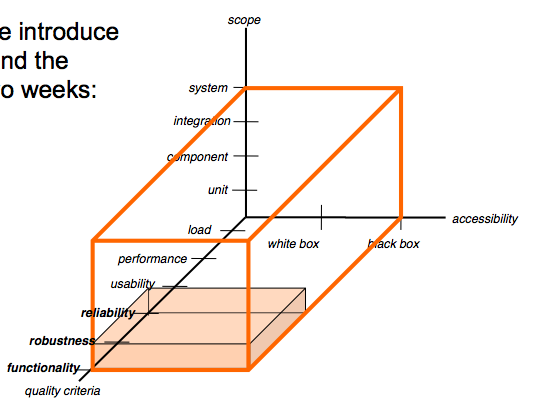
\includegraphics[scale=0.6]{unit_testing.png}

\subsection{Good Tests}
\begin{description}
	\item[Automatic] \hfill \\ ...invoking the tests and checking the results
	\item[Thorough] \hfill \\ ...test everything that is likely to break $\Ra$ Code coverage
	\item[Repeatable] \hfill \\ ...able to run over and over again, producing same results
	\item[Independent] \hfill \\  ...no test relies on an other test
	\item[Professional] \hfill \\ ...use same professional standards as for the production code
\end{description}

\subsection{Test Class}
A test class is responsible for testing a unit
\begin{itemize}
	\item Therefore, usually one test class is responsible for testing a single class
	\item A test class is a normal Java class. It can have fields, methods, constructors, inner classes...
	\item If the test class is declared in the same package as the class under test, then it can access its default and protected methods!
\end{itemize}
\subsection{Set Up}
In order to prepare each test, a setup method is called before each test method
\begin{itemize}
	\item In the setup method the test harness is initialized.
	\item The existence of a setup method guarantees, that each test method starts with exactly the same environment.
	\item A setup method must be public and is marked with the @Before annotation
\end{itemize}
\begin{lstlisting}
@Before
public void setup() {
	... 
}
\end{lstlisting}

\subsection{Test Method}
A unit test class consists of several test methods
\begin{itemize}
	\item Test methods take no arguments and return nothing, i.e. a test method is void
	\item Each test method should be completely independent of any other test method
	\item Often each test method tests a single method of the class under test. IDEs such as Eclipse support this pattern.
	\item A test method must be public and is marked with the @Test annotation.
\end{itemize}
\begin{lstlisting}
@Test
public void testY() {
	... 
}
\end{lstlisting}

\subsection{Tear Down}
After each test method, a tear down method is called.
\begin{itemize}
	\item The tear down method allows to tidy up the mess that was produced during the test method.
	\item The existence of teardown methods guarantees that the outcome of each test method can be cleaned up.
	\item A teardown method must be public an is marked with the @After annotation
\end{itemize}
\begin{lstlisting}
@After
public void teardown() {
	... 
}
\end{lstlisting}

\subsection{Assertions}
During each test method assertions are used to compare actual against expected results.
\begin{description}
	\item[assertEquals($<Type>$ expected, $<Type>$ actual)] \hfill
		\begin{itemize}
			\item Compares primitive types by value
			\item Compares class types by calling equals	
			\item Overloaded with all primitive types, Object and String.
		\end{itemize}
	\item[assertSame(Object expected, Object actual)] \hfill \\
		Compares references using ==-operator
	\item[assertNull(Object x), assertTrue(boolean b)] \hfill \\
		Does what it says :-)
	\item[fail()] \hfill \\
		Unconditional failure of test
\end{description}

\subsection{Exception}
Exceptions can also be tested. If only one exception is expected:
\begin{itemize}
	\item Use an expected argument to the @Test annotation
	\item @Test(expected=IllegalArgumentException.class)
\end{itemize}

\newpage
\section{Isolated Testing}

\subsection{Test doubles in Unit Testing}
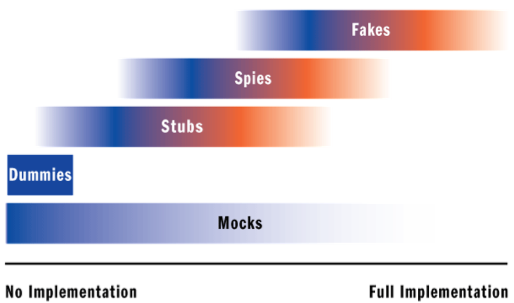
\includegraphics[scale=0.8]{test_doubles.png}
\begin{description}
	\item[Dummy] objects are passed around but never actually used. Usually they are just used to fill parameter lists.
	\item[Stubs] are minimal implementations of interfaces or base classes. Methods returning void will typically contain no implementation at all, while methods returning values will typically return hard-coded values.
	\item[Spys] similar to a stub, but a spy will also record which members were invoked so that unit tests can verify that members were invoked as expected.
	\item[Fakes] contain more complex implementations, typically handling interactions between different members of the type it's inheriting.
	\item[Mocks] objects pre-programmed with expectations which form a specification of the calls they are expected to receive.
\end{description}

\subsection{Mock Testing}
Mock objects simulate parts of the behavior of domain objects. Classes can be tested in isolation by simulating their collaborators with Mock Objects. Takes classes out of a natural environment and puts them in a well defined lab environment. \\
Use Mock Tests when:
\begin{itemize}
	\item The real object has non-deterministic behavior.
	\item The real object is difficult to set up.
	\item The real object is slow.
	\item The real object has a user interface.
	\item The test needs to ask the real object about how it was used
	\item The real object does not yet exist.
\end{itemize}
\begin{description}
	\item[Pros] \hfill
		\begin{itemize}
			\item Enforce the message that testing is about isolation
			\item Can simplify working with interfaces with many methods
			\item Can enable near-instant testing even of code that uses resource-bound APIs such as JDBC
		\end{itemize}
	\item[Cons] \hfill
		\begin{itemize}
			\item Can mirror the implementation too closely, making the test suite fragile	
			\item Mocking can become complex with APIs like JDBC
		\end{itemize}
\end{description}

\subsubsection{EasyMock}
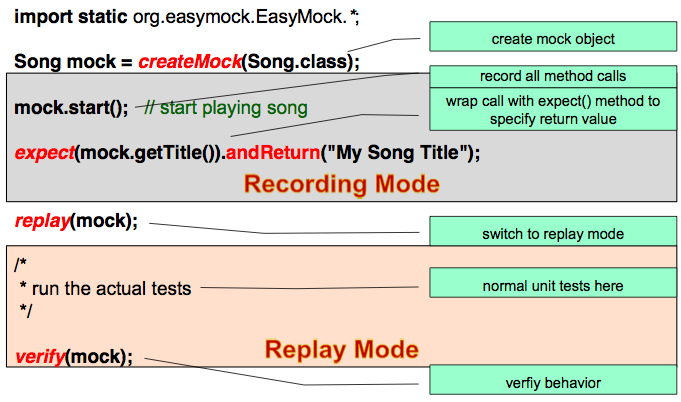
\includegraphics[scale=0.6]{easymock.png}

\newpage
\section{Software Quality Metrics}

\subsection{Software Metrics}
\begin{description}
	\item[Size Metrics] \hfill \\
		Lines of Code(LoC), Number of Statements, Fields, Methods, Packages
	\item[Dataflow Metrics] \hfill
		\begin{itemize}
			\item Cyclomatic Complexity (McCabe Complexity)
			\item Dead Code detection
			\item Initialization before use
		\end{itemize}
	\item[Style Metrics] \hfill 
		\begin{itemize}
			\item Number of Levels (nesting depth)
			\item Naming conventions, formatting conventions
		\end{itemize}
	\item[OO Metrics] \hfill
		\begin{itemize}
			\item No. of classes, packages, methods
			\item Inheritance depth / width
		\end{itemize}
	\item[Coupling Metrics] \hfill
		\begin{itemize}
			\item LCOM: lack of cohesion metrics
			\item No. of calling classes / no. of called classes
			\item Efferent / Afferent couplings
		\end{itemize}
	\item[Statistic Metrics] \hfill
		\begin{itemize}
			\item Instability
			\item Abstractness
		\end{itemize}
	\item[Performance Metrics (dynamic)] \hfill 
		\begin{itemize}
			\item Time spent
			\item Memory consumption (also memory leaks)
			\item Network traffic
			\item Bandwidth needed
			\item No. of clicks to perform a task
		\end{itemize}
\end{description}

\subsection{Cyclomatic Complexity}
Cyclomatic Complexity is the number of possible execution paths through the code. For a single method the Cyclomatic number N is defined as follows: N = b + 1 whereas b is the number of binary decision points (if, while, for, case ... ) \\
$N < 10 \Ra $ code well readable \\
Criticism: switch-statements are well readable but boost the cyclomatic number

\subsection{Cohesion and Coupling Metrics}
\begin{description}
	\item[Cohesion] \hfill \\
		Measure how closely related the methods of a class are.
	\item[Coupling / Dependency] \hfill \\
		Measure the degree to which each class relies on other classes
	\item Low coupling usually correlates with high cohesion
	\item Metrics: LCOM (Lack of Cohesion in Method)
\end{description}

\subsubsection{LCOM}
$LCOM^{HS} = \frac{m-avg(r(f))}{m}$
\begin{description}
	\item[Where] \hfill
		\begin{itemize}
			\item m is the number of methods of a class
			\item r(f) is the number of methods that access a field f
			\item Average r(f) over all fields.
		\end{itemize}
	\item[Examples] \hfill
		\begin{itemize}
			\item Each method accesses only one field \\
				$LCOM^{HS}$ = (almost) 1 low cohesion \\
				$\ra$ i.e. getters/setters are bad
			\item Each method reads all fields \\
				$LCOM^{HS}$ = 0 high cohesion
		\end{itemize}
\end{description}

\newpage
\section{Refactoring}
\begin{itemize}
	\item Refactoring improves the design of your system
	\item Refactoring makes your software easier to understand
	\item Refactoring helps you to find bugs
\end{itemize}
\Bold {Don't try to add features when wearing the refactoring hat.} \\ \\
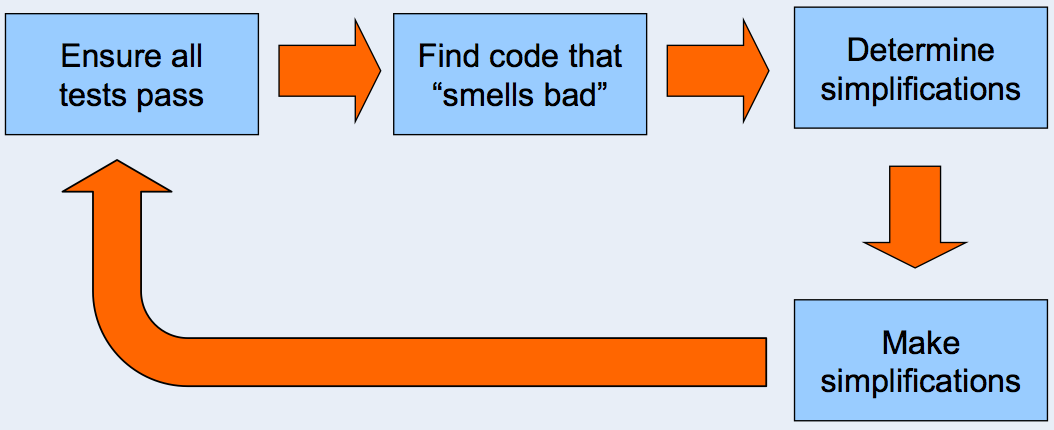
\includegraphics[scale=0.4]{refactoring_workflow.png}

\subsection{Problems}
\begin{itemize}
	\item Taken too far, refactoring can lead to incessant tinkering with the code, trying to make it perfect
	\item Databases can be difficult to refactor
	\item Refactoring published interfaces can cause problems for the code that uses those interfaces
\end{itemize}

\subsection{Code Smells}
\begin{description}
	\item[Too Much Code Smells] \hfill
		\begin{itemize}
			\item Duplicated Code
			\item Long Method	
			\item Large Class
			\item Long Parameter List
			\item Feature Envy
			\item Switch Statements
			\item Parallel Inheritance Hierarchies
		\end{itemize}
	\item[Not enough” Code Smells] \hfill 
		\begin{itemize}
			\item Empty Catch clause
		\end{itemize}
	\item[Code Change Smells] \hfill
		\begin{itemize}
			\item Divergent Change
			\item Shotgun Surgery	
		\end{itemize}
	\item[Comment Smells] \hfill 
		\begin{itemize}
			\item Need To Comment
			\item Too much Comments
		\end{itemize}
\end{description}

\newpage
\section{Coding Style \& Clean Code}
Clean code is simple and direct. Clean code reads like well-written prose. Clean code never obscures the designer’s intent but rather is full of crisp abstractions and straightforward lines of control. \\ \\
Code conventions usually cover: 
\begin{description}
	\item[Filenames and  File organization] \hfill 
		\begin{itemize}
			\item Names of files, directories
			\item Directory structure of project
			\item Structure of code files
		\end{itemize}
	\item[Indentation] \hfill
		\begin{itemize}
			\item Tabs vs. Spaces
			\item Line length
			\item Line Wrapping, line breaking rules	
		\end{itemize}
	\item[Naming Conventions] \hfill
		\begin{itemize}
			\item Naming conventions make programs more understandable by making them easier to read, to improve and to detect bugs
		\end{itemize}
	\item[Declarations, Statements and White Spaces] \hfill 
		\begin{itemize}
			\item How many variables shall be declared per line?
			\item Where shall variables be declared?
			\item How to indent e.g. a switch statement?
			\item Where to put block-braces \{ \}?
			\item Where to insert blank lines?
			\item Where to insert blank spaces in order to increase readability of expressions?
		\end{itemize}
\end{description}

\subsection{API Documentation}
API documentation is a contract between you and the clients of your code. It specifies the purpose of the class / interface and the functionality of the methods. Provide what is really needed, Remember that anything you provide, you are stuck with debugging, maintaining and updating.

\subsection{Class/Interface Documentation}
\begin{itemize}
	\item specifies the purpose and responsibility of the class/interface
	\item specifies important properties that cannot be expressed with the programming language (e.g. immutability, cloneability, singleton)
\end{itemize}

\subsection{Method Documentation}
\begin{itemize}
	\item specifies what you expect from the caller (preconditions \& parameters)
	\item specifies what you promise to give the caller in return (postconditions, invariants \& return values)	
\end{itemize}

\subsection{JavaDoc}
Javadoc is a separate program that comes with the JDK. It reads your program, makes lists of all the classes, interfaces, methods, and variables, and creates HTML pages displaying its results. \\
Write comments for the programmer who uses your classes: 
\begin{itemize}
	\item Anything you want to make available outside the class should be documented
	\item It is a good idea to describe, for your own use, private elements as well
\end{itemize}
javadoc can be set to generate documentation for:
\begin{itemize}
	\item only public elements
	\item public and protected elements
	\item public, protected, and package elements
	\item everything that is, public, protected, package, and private elements
\end{itemize}
javadoc comments must be immediately before:
\begin{itemize}
	\item a package (only in package-info.java)
	\item a class
	\item an interface
	\item a constructor
	\item a method	
	\item a field
\end{itemize}

\subsubsection{Tags In javadoc Comments}
\begin{description}
	\item[@param p] A description of parameter p.
	\item[@return] A description of the value returned (unless the method returns void).
	\item[@exception e] Describe any thrown exception.
	\item[@see] Adds a "See Also" heading with a link or text entry that points to reference
	\item[@author] your name
	\item[@version] a version number or date
\end{description}

\subsection{Programming Practices}
\begin{description}
	\item[No  Magic Numbers] \hfill
		\begin{itemize}
			\item Use named constants
		\end{itemize}
	\item[Do not optimize your code] \hfill 
		\begin{itemize}
			\item Variable assignment. Examples
			\item Do NOT (try to improve run-time performance): d = (a = b + c) + r;
		\end{itemize}
	\item[Know the boolean type] \hfill
		\begin{description}
			\item[poor:] if $(aBool == true)$ \{ return true; \} else \{ return false; \}
			\item[better:] $return (i < m) \&\& (j <= n);$
		\end{description}
	\item[Inappropriate Static] \hfill
		\begin{description}
			\item[poor:] ourlyPayCalculator.calculatePay(employee, overtimeRate)
			\item[better:] Math.max(double a, double b)
		\end{description}
	\item[Do one thing] \hfill
		\begin{itemize}
			\item A method should do only one thing
		\end{itemize}
	\item[Avoid negative conditionals] \hfill
		\begin{description}
			\item[poor:] if (!buffer.avoidCompaction())
			\item[better:] if (buffer.shouldCompact())
		\end{description}
	\item[Avoid Output Arguments] \hfill
		\begin{description}
			\item[poor:] appendFooter(report)
			\item[better:] report.appendFooter()
		\end{description}
\end{description}

\newpage
\section{Logging}
Logging is a technique for Monitoring and Debugging applications. \\
Debuggers focus on the state of a program now:
\begin{itemize}
	\item A stack trace can tell you only how the program got here directly
	\item It is not possible to detect what was before this actual ca
\end{itemize}
Logging provides information about the state of a program or a data structure over time:
\begin{itemize}
	\item Logging can reveal several classes of errors and information that debuggers cannot
\end{itemize}

\subsection{Benefits Using Logging Frameworks}
\begin{itemize}
	\item Configuration of the logging features is externalized
	\item Log messages can be prioritized
	\item Logging supports different message formats
	\item Enabling / disabling at runtime	
	\item Support different output targets
	\item Different output levels
	\item supports message caching in order to prevent performance decrease
\end{itemize}

\subsection{Concepts}
\begin{description}
	\item[Priority] Determines what is logged.
	\item[Level] Determines whether something is logged.
	\item[Appender] Determines where it is logged.
	\item[Layout] Determines how it is logged.
	\item[Logger] Writes a log entry to an appender in a given layout if the appropriate logging level is met by the priority of the log- instruction.
\end{description}

\subsection{Logging Levels}
\begin{description}
	\item[FATAL] In case of very severe errors from which your application cannot recover.
	\item[ERROR] When an error is encountered (but you application can still run).
	\item[WARN] Log requests to alert about harmful situations.
	\item[INFO] Logs to inform about progress of the application at a coarse grained level.
	\item[DEBUG] Log requests that are relevant to debug the application.
	\item[TRACE] Log on an extremely fined grained level to trace control flow.
\end{description}

\section{GUI- Testing}
\subsection{What does GUI Tests test?}
\subsubsection{Behavior of the GUI}
\begin{itemize}
\item Are the correct actions executed?
\item Are the actions correctly executed?
\item Is the navigation flow correct?
\item Does the GUI handle the data correctly?
\end{itemize}
\subsubsection{The state of the GUI}
\begin{itemize}
\item Does the GUI show the correct data?
\item Are the controls in the correct state ?
\end{itemize}

\subsection{How to do GUI-Testing}
\subsubsection{Manually}
\begin{itemize}
\item Done by manually stepping through many pages of test procedures.
(requires written test specs)
\item Very labor intensive, highly error prone.
\item Needs to be redone each time regression testing is required.
\item Very expensive
\end{itemize}
It is very hard to do manually tests systematically.

\subsubsection{Capture / Replay}
A capture replay tool is a set of software programs that captures user inputs and stores it into a format suitable to be used at a later time to replay the user inputs.\\

Major Drawback: If the GUI changes,you have to record a new set of user inputs.

\subsubsection{Scripting - In a seperate scripting language}
\textbf{\Bold Workflow:} $Writing Script \Longrightarrow SCRIPT \Longrightarrow REPLAY TOOL \Longrightarrow Execute Tests Automatically$

\begin{itemize}
\item Another programming language.
\item Needs to be subjected to some form of formal verification.
\item Eliminates human error during execution of the test.
\item Can be used (sometimes with modifications) for regression testing.
\item Different approaches for testing:
\item Spy gui controls
\item Image processing
\end{itemize}

\subsubsection{Integrated Test Framework (Unit Test Programming Style)}
\begin{itemize}
\item Scripting using the programming language of the productive code
\item Fully integrated into IDE
\item Easy and fast adaption of scripts
\item Typically runs with unit tests
\end{itemize}

\subsection{Writing testable GUI's}
An important aspect of test-driven development is writing software that is designed to be tested.\\
\\
Apply the guidelines for writing testable GUIs:
\begin{itemize}
\item Separate model (functionality) from view, moving as much code as possible away from the GUI.
\item Use a unique name for each GUI component to guarantee reliable component lookup.
\item Do not test default component behavior; for example, do not test that a button reacts to a mouse click -- that is the job of Oracle’s Swing team!
\item Concentrate on testing the expected behavior/state of your GUIs.
\end{itemize}

\subsection{FEST (GUI-Testing Tool)}
\begin{itemize}
\item A Collection of API’s for functional Swing GUI testing
\item Simulation of user-generated events and reliable GUI component lookup
\item Easy-to-use and powerful API that simplifies creation and maintenance of Swing GUI functional tests
\item Runs JUnit or TestNG test
\end{itemize}

\subsubsection{Workflow}
\begin{enumerate}
\item Create a setup method to create your own GUI instance (either frame or dialog)\\
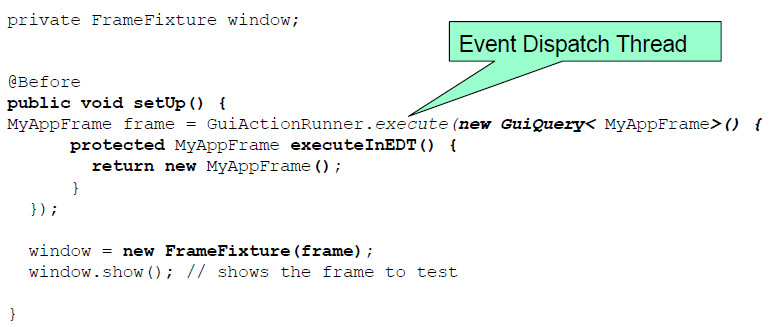
\includegraphics[scale=0.6]{FEST_Setup.png}

\item Close window and release resources\\
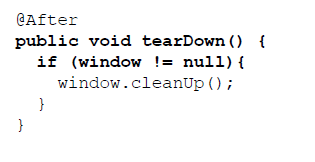
\includegraphics[scale=0.6]{FEST_CleanUP.png}
\newpage
\item Execute the actions on the controls
\item Verify expected behavior.\\
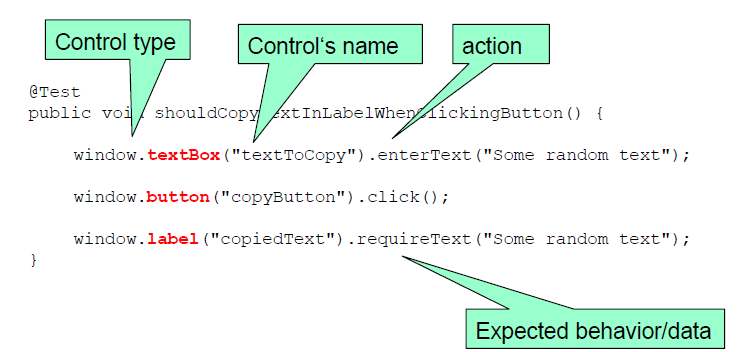
\includegraphics[scale=0.6]{FEST_Test.png}
\end{enumerate}







\end{document}